\documentclass[11pt]{article}
\usepackage{hyperref}
\usepackage{tabularx}
\usepackage{graphicx}
\usepackage{scalerel,stackengine}
\usepackage{adjustbox}
\usepackage{pdflscape}
\usepackage{rotating}
\stackMath
\newcommand\reallywidehat[1]{%
\savestack{\tmpbox}{\stretchto{%
  \scaleto{%
    \scalerel*[\widthof{\ensuremath{#1}}]{\kern-.6pt\bigwedge\kern-.6pt}%
    {\rule[-\textheight/2]{1ex}{\textheight}}%WIDTH-LIMITED BIG WEDGE
  }{\textheight}% 
}{0.5ex}}%
\stackon[1pt]{#1}{\tmpbox}%
}
\parskip 1ex
\graphicspath{ {./images/}}
%%%%%%%%%%%%%%%%%%%%%%%%%%%%%%%%%%%%%%%%%
% Lachaise Assignment
% Structure Specification File
% Version 1.0 (26/6/2018)
%
% This template originates from:
% http://www.LaTeXTemplates.com
%
% Authors:
% Marion Lachaise & François Févotte
% Vel (vel@LaTeXTemplates.com)
%
% License:
% CC BY-NC-SA 3.0 (http://creativecommons.org/licenses/by-nc-sa/3.0/)
% 
%%%%%%%%%%%%%%%%%%%%%%%%%%%%%%%%%%%%%%%%%

%----------------------------------------------------------------------------------------
%	PACKAGES AND OTHER DOCUMENT CONFIGURATIONS
%----------------------------------------------------------------------------------------

\usepackage{amsmath,amsfonts,stmaryrd,amssymb} % Math packages

\usepackage{enumerate} % Custom item numbers for enumerations

\usepackage[ruled]{algorithm2e} % Algorithms

\usepackage[framemethod=tikz]{mdframed} % Allows defining custom boxed/framed environments

\usepackage{listings} % File listings, with syntax highlighting
\lstset{
	basicstyle=\ttfamily, % Typeset listings in monospace font
}

%----------------------------------------------------------------------------------------
%	DOCUMENT MARGINS
%----------------------------------------------------------------------------------------

\usepackage{geometry} % Required for adjusting page dimensions and margins

\geometry{
	paper=a4paper, % Paper size, change to letterpaper for US letter size
	top=2.5cm, % Top margin
	bottom=3cm, % Bottom margin
	left=2.5cm, % Left margin
	right=2.5cm, % Right margin
	headheight=14pt, % Header height
	footskip=1.5cm, % Space from the bottom margin to the baseline of the footer
	headsep=1.2cm, % Space from the top margin to the baseline of the header
	%showframe, % Uncomment to show how the type block is set on the page
}

%----------------------------------------------------------------------------------------
%	FONTS
%----------------------------------------------------------------------------------------

\usepackage[utf8]{inputenc} % Required for inputting international characters
\usepackage[T1]{fontenc} % Output font encoding for international characters

\usepackage{XCharter} % Use the XCharter fonts

%----------------------------------------------------------------------------------------
%	COMMAND LINE ENVIRONMENT
%----------------------------------------------------------------------------------------

% Usage:
% \begin{commandline}
%	\begin{verbatim}
%		$ ls
%		
%		Applications	Desktop	...
%	\end{verbatim}
% \end{commandline}

\mdfdefinestyle{commandline}{
	leftmargin=pt,
	rightmargin=10pt,
	innerleftmargin=15pt,
	middlelinecolor=black!50!white,
	middlelinewidth=2pt,
	frametitlerule=false,
	backgroundcolor=black!5!white,
	frametitle={Command Line},
	frametitlefont={\normalfont\sffamily\color{white}\hspace{-1em}},
	frametitlebackgroundcolor=black!50!white,
	nobreak,
}

% Define a custom environment for command-line snapshots
\newenvironment{commandline}{
	\medskip
	\begin{mdframed}[style=commandline]
}{
	\end{mdframed}
	\medskip
}

%----------------------------------------------------------------------------------------
%	FILE CONTENTS ENVIRONMENT
%----------------------------------------------------------------------------------------

% Usage:
% \begin{file}[optional filename, defaults to "File"]
%	File contents, for example, with a listings environment
% \end{file}

\mdfdefinestyle{file}{
	innertopmargin=1.6\baselineskip,
	innerbottommargin=0.5\baselineskip,
	topline=false, bottomline=false,
	leftline=false, rightline=false,
	leftmargin=0cm,
	rightmargin=0cm,
	singleextra={%
		\draw[fill=black!10!white](P)++(0,-1.2em)rectangle(P-|O);
		\node[anchor=north west]
		at(P-|O){\ttfamily\mdfilename};
		%
		\def\l{3em}
		\draw(O-|P)++(-\l,0)--++(\l,\l)--(P)--(P-|O)--(O)--cycle;
		\draw(O-|P)++(-\l,0)--++(0,\l)--++(\l,0);
	},
	nobreak,
}

% Define a custom environment for file contents
\newenvironment{file}[1][File]{ % Set the default filename to "File"
	\medskip
	\newcommand{\mdfilename}{#1}
	\begin{mdframed}[style=file]
}{
	\end{mdframed}
	\medskip
}

%----------------------------------------------------------------------------------------
%	NUMBERED QUESTIONS ENVIRONMENT
%----------------------------------------------------------------------------------------

% Usage:
% \begin{question}[optional title]
%	Question contents
% \end{question}

\mdfdefinestyle{question}{
	innertopmargin=1.2\baselineskip,
	innerbottommargin=0.8\baselineskip,
	roundcorner=5pt,
	nobreak,
	singleextra={%
		\draw(P-|O)node[xshift=1em,anchor=west,fill=white,draw,rounded corners=5pt]{%
		Question \theQuestion\questionTitle};
	},
}

\newcounter{Question} % Stores the current question number that gets iterated with each new question

% Define a custom environment for numbered questions
\newenvironment{question}[1][\unskip]{
	\bigskip
	\stepcounter{Question}
	\newcommand{\questionTitle}{~#1}
	\begin{mdframed}[style=question]
}{
	\end{mdframed}
	\medskip
}

%----------------------------------------------------------------------------------------
%	WARNING TEXT ENVIRONMENT
%----------------------------------------------------------------------------------------

% Usage:
% \begin{warn}[optional title, defaults to "Warning:"]
%	Contents
% \end{warn}

\mdfdefinestyle{warning}{
	topline=false, bottomline=false,
	leftline=false, rightline=false,
	nobreak,
	singleextra={%
		\draw(P-|O)++(-0.5em,0)node(tmp1){};
		\draw(P-|O)++(0.5em,0)node(tmp2){};
		\fill[black,rotate around={45:(P-|O)}](tmp1)rectangle(tmp2);
		\node at(P-|O){\color{white}\scriptsize\bf !};
		\draw[very thick](P-|O)++(0,-1em)--(O);%--(O-|P);
	}
}

% Define a custom environment for warning text
\newenvironment{warn}[1][Warning:]{ % Set the default warning to "Warning:"
	\medskip
	\begin{mdframed}[style=warning]
		\noindent{\textbf{#1}}
}{
	\end{mdframed}
}

%----------------------------------------------------------------------------------------
%	INFORMATION ENVIRONMENT
%----------------------------------------------------------------------------------------

% Usage:
% \begin{info}[optional title, defaults to "Info:"]
% 	contents
% 	\end{info}

\mdfdefinestyle{info}{%
	topline=false, bottomline=false,
	leftline=false, rightline=false,
	nobreak,
	singleextra={%
		\fill[black](P-|O)circle[radius=0.4em];
		\node at(P-|O){\color{white}\scriptsize\bf i};
		\draw[very thick](P-|O)++(0,-0.8em)--(O);%--(O-|P);
	}
}

% Define a custom environment for information
\newenvironment{info}[1][Info:]{ % Set the default title to "Info:"
	\medskip
	\begin{mdframed}[style=info]
		\noindent{\textbf{#1}}
}{
	\end{mdframed}
}
 

\title{AMS 578 Spring 2021\\Multiple Regression Computing Project\\Preliminary Report}

\author{
  Kai Li\thanks{Department of Applied Mathematics and Statistics, Stony Brook University, email: \href{mailto:kai.li@stonybrook.edu}{kai.li@stonybrook.edu}}
}

\date{Stony Brook University --- \today}

\begin{document}
\maketitle

\section{Introduction}

Depression is one of the top five leading causes of disability and disease burden worldwide \cite{ar:caspi}. Researchers such as Caspi et al. \cite{ar:caspi} and Risch et al. \cite{ar:risch} have already conducted meta-analyses of the interaction between the serotonin transporter gene (5-HTTLPR) and stressful life events on the risk of depression using regression techniques. This multiple regression computing project aims to analyze a given synthetic dataset to fit a model using statistical software \texttt{R} given the background of related studies.

There are a few steps to perform a complete regression analysis. The first step is data summarizing and cleaning. Then, since variables can be nonlinear, checking if transformations are required is a key to ensure proper analysis and conclusion. An examination of important independent variables for the model becomes the following procedure. Especially, given a lack of consensus from the background, gene-by-environment and gene-by-gene interaction require additional inspection \cite{ar:caspi, ar:risch}. It is also given that at most four-way interactions of independent variables will appear. Finally, compare and determine if regression results are viable.

In this preliminary report, a summary statistics table will be provided as the first step of the analysis. Then, it is necessary to explain and use a methodology to deal with missing values if they exist in the data. Finally, a check on multicollinearity after coping with missing values enables to show if multicollinearity exists between variables. A complete model selection and analysis procedure will appear on the final report. 

\section{Summary Statistics}
To better understand and interpret a set of numerical data, it is easy to summarize the data by a few statistics representing its major characteristics, such as measures of location and dispersion \cite{bk:tamhane_dunlop}. \autoref{tab:summary} includes nine basic statistics for each variable. Note that there are 32 variables. Y is the quantitative independent variable measuring depressogenic effect; six environmental variables, denoted E1 through E6, quantify stressful life events; R1 through R25 are binary gene variables that are the candidate genes for depression from the serotonin system \cite{ar:caspi, ar:risch}. There are either 20 or 30 missing values for some of the variables in the dataset, about 1.08\% and 1.62\%, respectively, of the total observations.  Hence, an analysis of the missing data is needed.

\begin{table}[ht]
\centering
\begingroup\footnotesize
\caption{Summary Statistics Table} 
\label{tab:summary}
\begin{adjustbox}{width=\textwidth}
\begin{tabular}{lrrrrrrrrr}
 \textbf{Variable} & $\mathbf{n}$ & \textbf{Min} & $\mathbf{Q_1}$ & $\mathbf{\widetilde{x}}$ & $\mathbf{\bar{x}}$ & $\mathbf{Q_3}$ & \textbf{Max} & $\mathbf{s}$ & \textbf{\#NA} \\ 
  \hline
Y & 1848 & 6.11e+09 & 1.24e+10 & 1.44e+10 & 1.50e+10 & 1.66e+10 & 2.95e+10 & 3.86e+09 & 30 \\ 
  E1 & 1848 & 551.82 & 954.73 & 1072.67 & 1064.29 & 1174.55 & 1692.26 & 163.99 & 20 \\ 
  E2 & 1848 & 311.29 & 677.75 & 782.26 & 785.66 & 889.94 & 1298.12 & 158.01 & 30 \\ 
  E3 & 1848 & 215.87 & 576.02 & 683.49 & 683.07 & 785.42 & 1190.05 & 157.05 & 20 \\ 
  E4 & 1848 & -24.07 & 415.54 & 518.60 & 515.53 & 617.49 & 1053.83 & 158.21 & 20 \\ 
  E5 & 1848 & 223.00 & 710.97 & 822.30 & 822.87 & 932.60 & 1330.38 & 164.12 & 30 \\ 
  E6 & 1848 & 42.48 & 518.15 & 622.52 & 620.51 & 723.58 & 1225.55 & 159.18 & 20 \\ 
  R1 & 1848 & 0.00 & 0.00 & 0.00 & 0.49 & 1.00 & 1.00 & 0.50 & 30 \\ 
  R2 & 1848 & 0.00 & 0.00 & 1.00 & 0.52 & 1.00 & 1.00 & 0.50 & 30 \\ 
  R3 & 1848 & 0.00 & 0.00 & 1.00 & 0.52 & 1.00 & 1.00 & 0.50 & 30 \\ 
  R4 & 1848 & 0.00 & 0.00 & 1.00 & 0.52 & 1.00 & 1.00 & 0.50 & 30 \\ 
  R5 & 1848 & 0.00 & 0.00 & 1.00 & 0.51 & 1.00 & 1.00 & 0.50 &  0 \\ 
  R6 & 1848 & 0.00 & 0.00 & 1.00 & 0.51 & 1.00 & 1.00 & 0.50 &  0 \\ 
  R7 & 1848 & 0.00 & 0.00 & 1.00 & 0.51 & 1.00 & 1.00 & 0.50 &  0 \\ 
  R8 & 1848 & 0.00 & 0.00 & 0.00 & 0.50 & 1.00 & 1.00 & 0.50 &  0 \\ 
  R9 & 1848 & 0.00 & 0.00 & 1.00 & 0.51 & 1.00 & 1.00 & 0.50 &  0 \\ 
  R10 & 1848 & 0.00 & 0.00 & 0.00 & 0.50 & 1.00 & 1.00 & 0.50 &  0 \\ 
  R11 & 1848 & 0.00 & 0.00 & 0.00 & 0.50 & 1.00 & 1.00 & 0.50 & 30 \\ 
  R12 & 1818 & 0.00 & 0.00 & 0.00 & 0.50 & 1.00 & 1.00 & 0.50 & 30 \\ 
  R13 & 1848 & 0.00 & 0.00 & 0.00 & 0.50 & 1.00 & 1.00 & 0.50 &  0 \\ 
  R14 & 1848 & 0.00 & 0.00 & 0.00 & 0.48 & 1.00 & 1.00 & 0.50 &  0 \\ 
  R15 & 1848 & 0.00 & 0.00 & 0.00 & 0.49 & 1.00 & 1.00 & 0.50 &  0 \\ 
  R16 & 1848 & 0.00 & 0.00 & 1.00 & 0.51 & 1.00 & 1.00 & 0.50 &  0 \\ 
  R17 & 1848 & 0.00 & 0.00 & 0.00 & 0.50 & 1.00 & 1.00 & 0.50 & 30 \\ 
  R18 & 1848 & 0.00 & 0.00 & 1.00 & 0.51 & 1.00 & 1.00 & 0.50 &  0 \\ 
  R19 & 1848 & 0.00 & 0.00 & 1.00 & 0.52 & 1.00 & 1.00 & 0.50 &  0 \\ 
  R20 & 1848 & 0.00 & 0.00 & 1.00 & 0.50 & 1.00 & 1.00 & 0.50 &  0 \\ 
  R21 & 1848 & 0.00 & 0.00 & 1.00 & 0.51 & 1.00 & 1.00 & 0.50 & 30 \\ 
  R22 & 1848 & 0.00 & 0.00 & 1.00 & 0.50 & 1.00 & 1.00 & 0.50 &  0 \\ 
  R23 & 1848 & 0.00 & 0.00 & 0.00 & 0.49 & 1.00 & 1.00 & 0.50 & 30 \\ 
  R24 & 1848 & 0.00 & 0.00 & 1.00 & 0.50 & 1.00 & 1.00 & 0.50 &  0 \\ 
  R25 & 1848 & 0.00 & 0.00 & 1.00 & 0.50 & 1.00 & 1.00 & 0.50 & 30 \\ 
  \hline
\end{tabular}
\end{adjustbox}
\endgroup
\end{table}

\section{Missing Data Methodology}
In this section, a methodology to deal with the missing data will be discussed. Before that, the pattern of the missing values needs to be identified. In general, there are three types of missing data based on the patterns of missingness. Missing completely at random (MCAR) is defined as when the data missing probability is the same for all cases; missing at random (MAR) is defined as when the data missing probability is the same within the observed data alone; missing not at random (MNAR) is defined to be the data which is not MCAR or MAR \cite{bk:buuren, bk:rao}. There are available tools to visualize missing pattern. One is called the missing value specification plot, shown in \autoref{fig:vis_miss}. No systematic pattern of the missing values is observed from the plot. That is, the plot describes a general pattern with no specific structure, and hence the MCAR/MAR assumption is more likely to be true. Hypothesis testing can also be used to check for associations between missing and observed data. The null hypothesis is that the missing data is MCAR/MAR, versus the alternative hypothesis that it is MNAR. As shown in \autoref{tab:missing}, at the 0.01 level of significance, the test result is not significant, with Y being the dependent variable, environmental and gene as independent variables. In this project, the missing data will be considered MAR instead of MCAR because, for robustness, MCAR is an ideal but unreasonable assumption \cite{ar:kang}.

\begin{figure}[h!]
\begin{center}
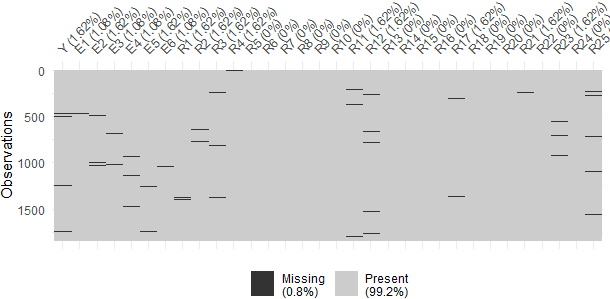
\includegraphics[scale=0.69]{vis_miss}
\end{center}
\caption{Missing Value Specification Plot}
\label{fig:vis_miss}
\end{figure}

After diagnosing the missing value pattern, it is appropriate to find a solution to deal with them. In many existing fields, multiple imputation is now accepted as the best general method to deal with datasets with missing values \cite{bk:buuren}. One significant advantage of multiple imputation, as opposed to single imputation, is that it preserves the natural variability of the missing data and incorporates the uncertainty due to the nature of MAR, which enables to perform a valid statistical inference \cite{ar:kang}. For this project, multivariate imputation by chained equations (MICE), a particular type of multiple imputation method, will be selected to impute the missing data. Because the dataset contains both continuous and binary variables, the chained equations approach is utilized due to its flexibility with variable types \cite{ar:azur}.

A package in \texttt{R} called \texttt{mice} corresponds directly to MICE techniques. The number of imputations created and the number of iterations for each imputation should be considered to use the method properly. Buuren \cite{bk:buuren} mentions that multiple imputation can generate unbiased estimates and correct confidence intervals with the number of imputed datasets as small as two. Raghunathan et al. \cite{bk:raghunathan} suggest 10 iterations per imputation. Given the size of the dataset, the amount of missing information, and the available computer resources, two imputed datasets and ten iterations for each will be outputted in this report \cite{ar:azur}.


\section{Multicollinearity Diagnostics}
Multiple regression models are used for a wide variety of applications. One common serious issue in regression analysis that may lead to a considerable decrease in the usefulness of a model is multicollinearity or near-linear dependence among regression variables \cite{bk:montgomery}. Currently, there are techniques for detecting multicollinearity. 

One informal measure of multicollinearity is the examination of the correlation matrix. Large coefficients of simple correlation coefficients between pairs of independent variables indicate a presence of serious multicollinearity \cite{bk:kutner}. That is, if the absolute value of a non-diagonal element, also called pairwise correlation, is close to 1, a nearly linearly dependent relationship between regressors is detected \cite{bk:montgomery}. The correlation matrices for the two imputed datasets are shown in \hyperref[tab:cormat1]{Tables 3} and \hyperref[tab:cormat2]{4}. All non-diagonal absolute pairwise correlation coefficients are less than or equal to 0.07, suggesting that the variables are not nearly linearly dependent.

Montgomery et al. \cite{bk:montgomery} also claim that when more than two independent variables are involved in a near-linear dependence relationship, it is not guaranteed that any of the pairwise correlations will be large. Thus, a formal way to diagnose multicollinearity is using variance inflation factor (VIF). If the largest VIF value among the regressors exceeds 10, it indicates multicollinearity, which can unduly influence model estimates \cite{bk:kutner}. The maximum VIFs in both datasets are 1.025 and 1.026, respectively, which suggests no multicollinearity issue in both imputed datasets.


\appendix
\section{Technical Implementation in \texttt{R}}
In the technical appendix, code implementation will be provided to show how results are obtained. At the beginning of the project, three files containing the unmerged datasets with variables \texttt{ID}, \texttt{Y}, \texttt{E}, and \texttt{R} are provided. The initial dataset is generated by combining the three files based on variable \texttt{ID}. Function \texttt{merge()} in \texttt{R} will work. Because there are numerous existing software/methods to merge datasets, the code for merging is omitted. The focus is the implementation of the combined data. The combined data is named variable \texttt{data} in the code below.

\subsection{Summary Statistics}
\autoref{tab:summary} is created using package \texttt{reporttools}, which directly outputs the summary statistics table in \LaTeX. Parts of summary statistics are omitted for simplicity purposes. 
\begin{file}[project.r]
\begin{lstlisting}[language = R]
library(reporttools)
vars0 <- with(data, data.frame(data[, -1]))
tableContinuous(vars = vars0, prec = 2, longtable = FALSE)
\end{lstlisting}
\end{file}

\subsection{Missing Value Specification Plot}
\autoref{fig:vis_miss} is a plot generated by package \texttt{naniar}. It provides functions to facilitate the plottings of missing values. \texttt{vis\_miss()} returns the missing value specification plot.
\begin{file}[project.r]
\begin{lstlisting}[language = R]
library(naniar)
vis_miss(data)
\end{lstlisting}
\end{file}

\subsection{Missing Data Pattern Analysis}
\texttt{finalfit} includes functions to ensure missing data is correctly identified. \texttt{missing\_compare()} performs the hypothesis testing of whether the missing data follows an MCAR/MAR or MNAR by comparing missing data in the dependent variable across explanatory variables. \autoref{tab:missing} shows the p-values in the return output. 
\begin{file}[project.r]
\begin{lstlisting}[language = R]
library(finalfit)
missing_compare(data, "Y", colnames(data)[-1])
\end{lstlisting}
\end{file}

\begin{table}[ht]
\centering
\begingroup\footnotesize
\caption{Missing Data Hypothesis Testing: Y} 
\label{tab:missing}
\begin{adjustbox}{width=\textwidth}
\begin{tabular}{lrrrr|lrrrr}
 \textbf{Variable} &  & \textbf{Not missing} & \textbf{Missing} & \textbf{p} & \textbf{Variable} &  & \textbf{Not missing} & \textbf{Missing} & \textbf{p}\\ 
  \hline
E1 & $\mathbf{\bar{x}}$ ($\mathbf{s}$) & 1063.2 (162.9) & 1134.3 (214.7) & 0.023 & E4 & $\mathbf{\bar{x}}$ ($\mathbf{s}$) & 515.1 (158.6) & 541.6 (131.2) & 0.371 \\
E2 & $\mathbf{\bar{x}}$ ($\mathbf{s}$) & 785.4 (157.8) & 801.0 (169.9) & 0.591 & E5 & $\mathbf{\bar{x}}$ ($\mathbf{s}$) & 823.0 (164.2) & 815.7 (160.3) & 0.816 \\
E3 & $\mathbf{\bar{x}}$ ($\mathbf{s}$) & 683.6 (156.6) & 650.3 (183.6) & 0.257 & E6 & $\mathbf{\bar{x}}$ ($\mathbf{s}$) & 620.5 (159.3) & 622.2 (153.2) & 0.954 \\
\hline
R1 & 0 & 910 (98.5) & 14 (1.5) & 0.929 & R14 & 0 & 936 (98.3) & 16 (1.7) & 0.987 \\
   & 1 & 879 (98.3) & 15 (1.7) &  &  & 1 & 882 (98.4) & 14 (1.6) &  \\
R2 & 0 & 855 (98.5) & 13 (1.5) & 0.762 & R15 & 0 & 937 (98.5) & 14 (1.5) & 0.730 \\
   & 1 & 933 (98.2) & 17 (1.8) &  &  & 1 & 881 (98.2) & 16 (1.8) &  \\
R3 & 0 & 851 (98.4) & 14 (1.6) & 1.000 & R16 & 0 & 893 (98.0) & 18 (2.0) & 0.318 \\
   & 1 & 937 (98.3) & 16 (1.7) &  &  & 1 & 925 (98.7) & 12 (1.3) &  \\
R4 & 0 & 862 (98.6) & 12 (1.4) & 0.479 & R17 & 0 & 900 (98.7) & 12 (1.3) & 0.443 \\
   & 1 & 926 (98.1) & 18 (1.9) &  &  & 1 & 889 (98.1) & 17 (1.9) &  \\
R5 & 0 & 885 (98.1) & 17 (1.9) & 0.494 & R18 & 0 & 886 (97.9) & 19 (2.1) & 0.161 \\
   & 1 & 933 (98.6) & 13 (1.4) &  &  & 1 & 932 (98.8) & 11 (1.2) &  \\
R6 & 0 & 893 (98.1) & 17 (1.9) & 0.525 & R19 & 0 & 870 (98.2) & 16 (1.8) & 0.681 \\
   & 1 & 925 (98.6) & 13 (1.4) &  &  & 1 & 948 (98.5) & 14 (1.5) &  \\
R7 & 0 & 890 (98.7) & 12 (1.3) & 0.430 & R20 & 0 & 905 (98.4) & 15 (1.6) & 1.000 \\
   & 1 & 928 (98.1) & 18 (1.9) &  &  & 1 & 913 (98.4) & 15 (1.6) &  \\
R8 & 0 & 908 (98.2) & 17 (1.8) & 0.585 & R21 & 0 & 877 (98.7) & 12 (1.3) & 0.424 \\
   & 1 & 910 (98.6) & 13 (1.4) &  &  & 1 & 911 (98.1) & 18 (1.9) &  \\
R9 & 0 & 898 (98.6) & 13 (1.4) & 0.635 & R22 & 0 & 902 (98.3) & 16 (1.7) & 0.826 \\
   & 1 & 920 (98.2) & 17 (1.8) &  &  & 1 & 916 (98.5) & 14 (1.5) &  \\
R10 & 0 & 906 (97.9) & 19 (2.1) & 0.200 & R23 & 0 & 914 (98.5) & 14 (1.5) & 0.910 \\
    & 1 & 912 (98.8) & 11 (1.2) &  &  & 1 & 875 (98.3) & 15 (1.7) &  \\
R11 & 0 & 903 (98.6) & 13 (1.4) & 0.552 & R24 & 0 & 906 (98.2) & 17 (1.8) & 0.577 \\
    & 1 & 885 (98.1) & 17 (1.9) &  &  & 1 & 912 (98.6) & 13 (1.4) &  \\
R12 & 0 & 896 (98.1) & 17 (1.9) & 0.469 & R25 & 0 & 886 (98.0) & 18 (2.0) & 0.342 \\
    & 1 & 893 (98.7) & 12 (1.3) &  &  & 1 & 902 (98.7) & 12 (1.3) &  \\
R13 & 0 & 919 (98.5) & 14 (1.5) & 0.812\\
    & 1 & 899 (98.3) & 16 (1.7) &      \\
  \hline
\end{tabular}
\end{adjustbox}
\endgroup
\end{table}

\subsection{Multiple Imputation}
Package \texttt{mice}, written by Karin Groothuis-Oudshoorn and Van Buuren, can perform multiple imputation computations \cite{bk:buuren}. The imputation method selected for each dataset is classification and regression trees (CART). Function \texttt{mice()} generates multiple imputation datasets, and function \texttt{complete()} returns the complete data in a specified format. After that, each complete dataset is ready to perform analysis. 
\begin{file}[project.r]
\begin{lstlisting}[language = R]
library(mice)
imp <- mice(data, method = "cart", m = 2, maxit = 10,
            seed = 123, print = FALSE)
data1 <- complete(imp, 1)
data2 <- complete(imp, 2)
\end{lstlisting}
\end{file}

\subsection{Multicollinearity Diagnostics}
Correlation matrices in \hyperref[tab:cormat1]{Tables 3} and \hyperref[tab:cormat2]{4} can be obtained using function \texttt{cor()}. The correlation coefficients are rounded to 2 decimals to reduce the unnecessary digits. VIFs can be calculated under package \texttt{car} for linear models. Function \texttt{vif()} outputs VIF values for all variables in linear regression model \texttt{lm()}. Because only the maximums are considered, return using function \texttt{max()} is sufficient.

\setcounter{MaxMatrixCols}{32}
\begin{landscape}
% latex table generated in R 3.6.3 by xtable 1.8-4 package
% Fri Apr 16 21:14:32 2021
\begin{table}[ht]
\centering
\begingroup\footnotesize
\caption{Correlation Matrix for Dataset 1} 
\label{tab:cormat1}
\begin{adjustbox}{width=\linewidth, height=7.75cm}
\begin{tabular}{rrrrrrrrrrrrrrrrrrrrrrrrrrrrrrrrr}
  \hline
 & E1 & E2 & E3 & E4 & E5 & E6 & R1 & R2 & R3 & R4 & R5 & R6 & R7 & R8 & R9 & R10 & R11 & R12 & R13 & R14 & R15 & R16 & R17 & R18 & R19 & R20 & R21 & R22 & R23 & R24 & R25 \\ 
  \hline
  E1 & 1.00 & -0.01 & 0.00 & 0.00 & 0.02 & -0.01 & 0.04 & 0.03 & 0.02 & -0.04 & 0.01 & 0.01 & -0.00 & -0.01 & -0.00 & -0.03 & -0.00 & 0.01 & -0.01 & -0.01 & 0.00 & -0.02 & -0.01 & 0.01 & -0.01 & 0.01 & 0.03 & -0.02 & 0.05 & 0.00 & -0.01 \\ 
  E2 & -0.01 & 1.00 & 0.05 & 0.01 & -0.03 & -0.01 & 0.00 & 0.02 & -0.01 & -0.05 & -0.02 & 0.02 & 0.01 & -0.02 & -0.02 & -0.01 & 0.01 & 0.01 & -0.01 & -0.02 & 0.02 & 0.00 & 0.00 & -0.01 & 0.01 & -0.01 & -0.02 & 0.03 & -0.00 & -0.01 & 0.04 \\ 
  E3 & 0.00 & 0.05 & 1.00 & -0.03 & -0.01 & -0.02 & -0.00 & -0.01 & 0.02 & -0.02 & 0.02 & -0.01 & -0.00 & 0.00 & -0.00 & 0.02 & -0.01 & 0.04 & 0.03 & 0.03 & -0.00 & 0.04 & 0.01 & 0.03 & -0.02 & -0.01 & 0.02 & 0.00 & 0.00 & 0.00 & 0.01 \\ 
  E4 & 0.00 & 0.01 & -0.03 & 1.00 & 0.01 & -0.01 & 0.02 & 0.01 & 0.02 & -0.03 & -0.04 & -0.01 & 0.00 & 0.00 & -0.01 & 0.02 & 0.04 & -0.04 & -0.05 & 0.00 & -0.02 & -0.02 & 0.01 & -0.01 & 0.03 & 0.03 & -0.00 & 0.01 & 0.02 & 0.01 & 0.01 \\ 
  E5 & 0.02 & -0.03 & -0.01 & 0.01 & 1.00 & 0.00 & 0.02 & 0.04 & 0.04 & 0.01 & 0.02 & 0.01 & -0.01 & -0.04 & 0.02 & -0.01 & -0.06 & 0.03 & 0.06 & 0.01 & 0.02 & 0.02 & -0.04 & -0.04 & -0.03 & -0.01 & 0.01 & -0.00 & 0.01 & 0.00 & 0.06 \\ 
  E6 & -0.01 & -0.01 & -0.02 & -0.01 & 0.00 & 1.00 & -0.04 & -0.01 & 0.01 & -0.03 & 0.01 & -0.01 & 0.01 & -0.01 & 0.03 & 0.03 & 0.02 & -0.01 & 0.00 & 0.00 & -0.03 & -0.00 & -0.02 & -0.06 & -0.03 & 0.04 & 0.01 & -0.02 & -0.01 & -0.06 & -0.03 \\ 
  R1 & 0.04 & 0.00 & -0.00 & 0.02 & 0.02 & -0.04 & 1.00 & 0.06 & -0.02 & 0.01 & 0.01 & 0.00 & 0.03 & -0.02 & 0.04 & 0.04 & 0.03 & 0.01 & 0.03 & -0.01 & -0.03 & -0.03 & 0.04 & 0.00 & 0.04 & -0.01 & 0.01 & 0.01 & 0.01 & 0.02 & -0.01 \\ 
  R2 & 0.03 & 0.02 & -0.01 & 0.01 & 0.04 & -0.01 & 0.06 & 1.00 & -0.01 & 0.04 & -0.01 & 0.01 & 0.01 & -0.02 & -0.00 & 0.04 & 0.04 & 0.04 & 0.01 & -0.06 & -0.00 & -0.03 & 0.01 & -0.04 & 0.04 & -0.00 & -0.00 & -0.02 & 0.03 & 0.01 & -0.00 \\ 
  R3 & 0.02 & -0.01 & 0.02 & 0.02 & 0.04 & 0.01 & -0.02 & -0.01 & 1.00 & 0.04 & 0.01 & -0.00 & 0.01 & -0.03 & -0.05 & -0.05 & -0.00 & -0.02 & -0.03 & -0.01 & -0.03 & -0.01 & 0.02 & 0.01 & -0.06 & 0.03 & 0.01 & 0.02 & 0.01 & 0.02 & -0.01 \\ 
  R4 & -0.04 & -0.05 & -0.02 & -0.03 & 0.01 & -0.03 & 0.01 & 0.04 & 0.04 & 1.00 & -0.01 & -0.00 & -0.01 & 0.03 & -0.00 & 0.03 & -0.03 & -0.01 & -0.03 & 0.00 & -0.01 & 0.01 & 0.01 & -0.00 & 0.02 & 0.01 & -0.01 & -0.02 & 0.01 & 0.01 & 0.01 \\ 
  R5 & 0.01 & -0.02 & 0.02 & -0.04 & 0.02 & 0.01 & 0.01 & -0.01 & 0.01 & -0.01 & 1.00 & 0.00 & 0.02 & 0.01 & -0.01 & -0.01 & -0.04 & -0.02 & -0.01 & 0.04 & 0.00 & -0.01 & -0.04 & -0.03 & 0.01 & -0.01 & 0.01 & -0.02 & -0.02 & 0.02 & 0.04 \\ 
  R6 & 0.01 & 0.02 & -0.01 & -0.01 & 0.01 & -0.01 & 0.00 & 0.01 & -0.00 & -0.00 & 0.00 & 1.00 & 0.02 & -0.01 & -0.00 & 0.03 & 0.01 & 0.02 & 0.04 & -0.03 & 0.01 & 0.02 & -0.01 & 0.01 & 0.00 & -0.02 & -0.02 & -0.01 & -0.01 & 0.02 & -0.03 \\ 
  R7 & -0.00 & 0.01 & -0.00 & 0.00 & -0.01 & 0.01 & 0.03 & 0.01 & 0.01 & -0.01 & 0.02 & 0.02 & 1.00 & 0.01 & 0.01 & 0.04 & -0.01 & -0.01 & -0.00 & 0.01 & -0.05 & 0.00 & -0.01 & -0.02 & -0.01 & -0.02 & 0.00 & 0.03 & -0.01 & -0.01 & -0.01 \\ 
  R8 & -0.01 & -0.02 & 0.00 & 0.00 & -0.04 & -0.01 & -0.02 & -0.02 & -0.03 & 0.03 & 0.01 & -0.01 & 0.01 & 1.00 & -0.03 & 0.00 & 0.05 & 0.02 & 0.01 & -0.01 & -0.01 & 0.05 & 0.01 & 0.01 & -0.02 & -0.02 & -0.00 & -0.00 & -0.01 & -0.04 & -0.04 \\ 
  R9 & -0.00 & -0.02 & -0.00 & -0.01 & 0.02 & 0.03 & 0.04 & -0.00 & -0.05 & -0.00 & -0.01 & -0.00 & 0.01 & -0.03 & 1.00 & 0.06 & 0.00 & 0.01 & -0.01 & -0.01 & -0.00 & -0.04 & 0.05 & 0.01 & -0.00 & 0.01 & 0.01 & 0.00 & -0.00 & -0.01 & 0.02 \\ 
  R10 & -0.03 & -0.01 & 0.02 & 0.02 & -0.01 & 0.03 & 0.04 & 0.04 & -0.05 & 0.03 & -0.01 & 0.03 & 0.04 & 0.00 & 0.06 & 1.00 & 0.02 & -0.04 & -0.02 & 0.02 & -0.02 & -0.02 & 0.02 & -0.00 & 0.05 & -0.02 & -0.01 & 0.01 & -0.01 & -0.02 & 0.03 \\ 
  R11 & -0.00 & 0.01 & -0.01 & 0.04 & -0.06 & 0.02 & 0.03 & 0.04 & -0.00 & -0.03 & -0.04 & 0.01 & -0.01 & 0.05 & 0.00 & 0.02 & 1.00 & -0.02 & -0.04 & 0.02 & -0.02 & -0.01 & 0.01 & 0.01 & -0.01 & -0.02 & 0.06 & -0.03 & -0.00 & -0.02 & -0.02 \\ 
  R12 & 0.01 & 0.01 & 0.04 & -0.04 & 0.03 & -0.01 & 0.01 & 0.04 & -0.02 & -0.01 & -0.02 & 0.02 & -0.01 & 0.02 & 0.01 & -0.04 & -0.02 & 1.00 & 0.01 & -0.00 & 0.01 & -0.02 & -0.01 & 0.02 & 0.01 & -0.01 & -0.01 & 0.02 & -0.03 & 0.01 & -0.00 \\ 
  R13 & -0.01 & -0.01 & 0.03 & -0.05 & 0.06 & 0.00 & 0.03 & 0.01 & -0.03 & -0.03 & -0.01 & 0.04 & -0.00 & 0.01 & -0.01 & -0.02 & -0.04 & 0.01 & 1.00 & 0.00 & -0.01 & 0.04 & -0.01 & -0.06 & 0.00 & -0.01 & -0.02 & 0.02 & -0.02 & -0.03 & 0.00 \\ 
  R14 & -0.01 & -0.02 & 0.03 & 0.00 & 0.01 & 0.00 & -0.01 & -0.06 & -0.01 & 0.00 & 0.04 & -0.03 & 0.01 & -0.01 & -0.01 & 0.02 & 0.02 & -0.00 & 0.00 & 1.00 & 0.01 & 0.02 & -0.00 & 0.01 & -0.00 & -0.03 & 0.00 & 0.04 & 0.03 & 0.01 & -0.00 \\ 
  R15 & 0.00 & 0.02 & -0.00 & -0.02 & 0.02 & -0.03 & -0.03 & -0.00 & -0.03 & -0.01 & 0.00 & 0.01 & -0.05 & -0.01 & -0.00 & -0.02 & -0.02 & 0.01 & -0.01 & 0.01 & 1.00 & 0.01 & 0.01 & 0.01 & 0.00 & 0.02 & -0.01 & -0.02 & 0.05 & 0.01 & 0.01 \\ 
  R16 & -0.02 & 0.00 & 0.04 & -0.02 & 0.02 & -0.00 & -0.03 & -0.03 & -0.01 & 0.01 & -0.01 & 0.02 & 0.00 & 0.05 & -0.04 & -0.02 & -0.01 & -0.02 & 0.04 & 0.02 & 0.01 & 1.00 & 0.04 & -0.03 & -0.01 & 0.03 & -0.03 & -0.02 & 0.02 & -0.05 & -0.00 \\ 
  R17 & -0.01 & 0.00 & 0.01 & 0.01 & -0.04 & -0.02 & 0.04 & 0.01 & 0.02 & 0.01 & -0.04 & -0.01 & -0.01 & 0.01 & 0.05 & 0.02 & 0.01 & -0.01 & -0.01 & -0.00 & 0.01 & 0.04 & 1.00 & -0.01 & 0.00 & 0.00 & -0.01 & 0.00 & 0.00 & 0.01 & 0.06 \\ 
  R18 & 0.01 & -0.01 & 0.03 & -0.01 & -0.04 & -0.06 & 0.00 & -0.04 & 0.01 & -0.00 & -0.03 & 0.01 & -0.02 & 0.01 & 0.01 & -0.00 & 0.01 & 0.02 & -0.06 & 0.01 & 0.01 & -0.03 & -0.01 & 1.00 & 0.05 & 0.04 & 0.03 & -0.01 & 0.02 & -0.01 & -0.03 \\ 
  R19 & -0.01 & 0.01 & -0.02 & 0.03 & -0.03 & -0.03 & 0.04 & 0.04 & -0.06 & 0.02 & 0.01 & 0.00 & -0.01 & -0.02 & -0.00 & 0.05 & -0.01 & 0.01 & 0.00 & -0.00 & 0.00 & -0.01 & 0.00 & 0.05 & 1.00 & 0.00 & -0.01 & -0.00 & 0.00 & -0.03 & -0.03 \\ 
  R20 & 0.01 & -0.01 & -0.01 & 0.03 & -0.01 & 0.04 & -0.01 & -0.00 & 0.03 & 0.01 & -0.01 & -0.02 & -0.02 & -0.02 & 0.01 & -0.02 & -0.02 & -0.01 & -0.01 & -0.03 & 0.02 & 0.03 & 0.00 & 0.04 & 0.00 & 1.00 & 0.06 & -0.03 & -0.04 & -0.01 & 0.01 \\ 
  R21 & 0.03 & -0.02 & 0.02 & -0.00 & 0.01 & 0.01 & 0.01 & -0.00 & 0.01 & -0.01 & 0.01 & -0.02 & 0.00 & -0.00 & 0.01 & -0.01 & 0.06 & -0.01 & -0.02 & 0.00 & -0.01 & -0.03 & -0.01 & 0.03 & -0.01 & 0.06 & 1.00 & -0.01 & -0.02 & 0.01 & -0.00 \\ 
  R22 & -0.02 & 0.03 & 0.00 & 0.01 & -0.00 & -0.02 & 0.01 & -0.02 & 0.02 & -0.02 & -0.02 & -0.01 & 0.03 & -0.00 & 0.00 & 0.01 & -0.03 & 0.02 & 0.02 & 0.04 & -0.02 & -0.02 & 0.00 & -0.01 & -0.00 & -0.03 & -0.01 & 1.00 & -0.01 & -0.03 & 0.03 \\ 
  R23 & 0.05 & -0.00 & 0.00 & 0.02 & 0.01 & -0.01 & 0.01 & 0.03 & 0.01 & 0.01 & -0.02 & -0.01 & -0.01 & -0.01 & -0.00 & -0.01 & -0.00 & -0.03 & -0.02 & 0.03 & 0.05 & 0.02 & 0.00 & 0.02 & 0.00 & -0.04 & -0.02 & -0.01 & 1.00 & 0.02 & 0.04 \\ 
  R24 & 0.00 & -0.01 & 0.00 & 0.01 & 0.00 & -0.06 & 0.02 & 0.01 & 0.02 & 0.01 & 0.02 & 0.02 & -0.01 & -0.04 & -0.01 & -0.02 & -0.02 & 0.01 & -0.03 & 0.01 & 0.01 & -0.05 & 0.01 & -0.01 & -0.03 & -0.01 & 0.01 & -0.03 & 0.02 & 1.00 & 0.02 \\ 
  R25 & -0.01 & 0.04 & 0.01 & 0.01 & 0.06 & -0.03 & -0.01 & -0.00 & -0.01 & 0.01 & 0.04 & -0.03 & -0.01 & -0.04 & 0.02 & 0.03 & -0.02 & -0.00 & 0.00 & -0.00 & 0.01 & -0.00 & 0.06 & -0.03 & -0.03 & 0.01 & -0.00 & 0.03 & 0.04 & 0.02 & 1.00 \\ 
   \hline
\end{tabular}
\end{adjustbox}
\endgroup
\end{table}

% latex table generated in R 3.6.3 by xtable 1.8-4 package
% Fri Apr 16 22:00:59 2021
\begin{table}[ht]
\centering
\begingroup\footnotesize
\caption{Correlation Matrix for Dataset 2} 
\label{tab:cormat2}
\begin{adjustbox}{width=\linewidth, height=7.75cm}
\begin{tabular}{rrrrrrrrrrrrrrrrrrrrrrrrrrrrrrrrr}
  \hline
 & E1 & E2 & E3 & E4 & E5 & E6 & R1 & R2 & R3 & R4 & R5 & R6 & R7 & R8 & R9 & R10 & R11 & R12 & R13 & R14 & R15 & R16 & R17 & R18 & R19 & R20 & R21 & R22 & R23 & R24 & R25 \\ 
  \hline
  E1 & 1.00 & -0.02 & -0.00 & 0.00 & 0.02 & -0.01 & 0.03 & 0.03 & 0.03 & -0.04 & 0.01 & 0.01 & -0.00 & -0.01 & -0.00 & -0.03 & -0.00 & 0.01 & -0.01 & -0.01 & 0.01 & -0.02 & -0.01 & 0.01 & -0.01 & 0.01 & 0.03 & -0.02 & 0.06 & 0.00 & -0.01 \\ 
  E2 & -0.02 & 1.00 & 0.05 & 0.01 & -0.02 & -0.01 & -0.00 & 0.02 & -0.02 & -0.05 & -0.01 & 0.01 & 0.01 & -0.02 & -0.01 & -0.02 & 0.00 & 0.02 & -0.00 & -0.02 & 0.02 & 0.01 & -0.01 & -0.01 & 0.01 & -0.00 & -0.01 & 0.03 & -0.01 & -0.01 & 0.04 \\ 
  E3 & -0.00 & 0.05 & 1.00 & -0.03 & -0.01 & -0.03 & 0.00 & -0.01 & 0.03 & -0.03 & 0.02 & -0.01 & -0.00 & -0.00 & 0.00 & 0.02 & -0.00 & 0.05 & 0.03 & 0.03 & 0.00 & 0.05 & 0.02 & 0.03 & -0.02 & -0.01 & 0.01 & 0.00 & -0.00 & 0.00 & 0.01 \\ 
  E4 & 0.00 & 0.01 & -0.03 & 1.00 & 0.01 & -0.01 & 0.02 & 0.01 & 0.02 & -0.02 & -0.04 & -0.01 & 0.00 & -0.00 & -0.01 & 0.02 & 0.03 & -0.04 & -0.05 & 0.01 & -0.02 & -0.02 & 0.01 & -0.01 & 0.03 & 0.03 & -0.01 & 0.01 & 0.03 & 0.01 & 0.01 \\ 
  E5 & 0.02 & -0.02 & -0.01 & 0.01 & 1.00 & -0.01 & 0.02 & 0.03 & 0.05 & 0.01 & 0.03 & 0.01 & -0.01 & -0.04 & 0.02 & -0.01 & -0.06 & 0.03 & 0.06 & 0.01 & 0.02 & 0.02 & -0.04 & -0.04 & -0.03 & -0.01 & 0.02 & -0.00 & 0.00 & 0.01 & 0.07 \\ 
  E6 & -0.01 & -0.01 & -0.03 & -0.01 & -0.01 & 1.00 & -0.05 & -0.01 & 0.01 & -0.04 & 0.01 & -0.01 & -0.00 & -0.01 & 0.02 & 0.03 & 0.02 & -0.01 & 0.00 & 0.01 & -0.03 & -0.00 & -0.02 & -0.06 & -0.03 & 0.04 & 0.01 & -0.03 & -0.02 & -0.05 & -0.02 \\ 
  R1 & 0.03 & -0.00 & 0.00 & 0.02 & 0.02 & -0.05 & 1.00 & 0.06 & -0.02 & 0.01 & 0.02 & -0.00 & 0.02 & -0.02 & 0.05 & 0.04 & 0.04 & 0.02 & 0.02 & -0.01 & -0.03 & -0.03 & 0.04 & 0.00 & 0.04 & -0.01 & 0.02 & 0.01 & -0.01 & 0.02 & -0.02 \\ 
  R2 & 0.03 & 0.02 & -0.01 & 0.01 & 0.03 & -0.01 & 0.06 & 1.00 & -0.00 & 0.05 & -0.00 & 0.01 & 0.01 & -0.02 & -0.01 & 0.03 & 0.04 & 0.05 & 0.01 & -0.05 & -0.00 & -0.03 & 0.01 & -0.05 & 0.05 & -0.01 & -0.00 & -0.01 & 0.03 & 0.00 & 0.01 \\ 
  R3 & 0.03 & -0.02 & 0.03 & 0.02 & 0.05 & 0.01 & -0.02 & -0.00 & 1.00 & 0.04 & 0.01 & -0.01 & 0.01 & -0.03 & -0.05 & -0.05 & -0.00 & -0.02 & -0.03 & 0.00 & -0.03 & -0.01 & 0.01 & 0.01 & -0.05 & 0.02 & 0.00 & 0.02 & 0.01 & 0.03 & -0.02 \\ 
  R4 & -0.04 & -0.05 & -0.03 & -0.02 & 0.01 & -0.04 & 0.01 & 0.05 & 0.04 & 1.00 & -0.01 & -0.00 & -0.01 & 0.04 & 0.01 & 0.04 & -0.03 & -0.01 & -0.03 & -0.00 & -0.02 & 0.01 & 0.01 & 0.01 & 0.02 & 0.01 & -0.01 & -0.02 & 0.01 & 0.01 & 0.01 \\ 
  R5 & 0.01 & -0.01 & 0.02 & -0.04 & 0.03 & 0.01 & 0.02 & -0.00 & 0.01 & -0.01 & 1.00 & 0.00 & 0.02 & 0.01 & -0.01 & -0.01 & -0.05 & -0.02 & -0.01 & 0.04 & 0.00 & -0.01 & -0.05 & -0.03 & 0.01 & -0.01 & 0.01 & -0.02 & -0.02 & 0.02 & 0.05 \\ 
  R6 & 0.01 & 0.01 & -0.01 & -0.01 & 0.01 & -0.01 & -0.00 & 0.01 & -0.01 & -0.00 & 0.00 & 1.00 & 0.02 & -0.01 & -0.00 & 0.03 & 0.00 & 0.02 & 0.04 & -0.03 & 0.01 & 0.02 & -0.00 & 0.01 & 0.00 & -0.02 & -0.02 & -0.01 & -0.01 & 0.02 & -0.03 \\ 
  R7 & -0.00 & 0.01 & -0.00 & 0.00 & -0.01 & -0.00 & 0.02 & 0.01 & 0.01 & -0.01 & 0.02 & 0.02 & 1.00 & 0.01 & 0.01 & 0.04 & -0.01 & -0.01 & -0.00 & 0.01 & -0.05 & 0.00 & -0.01 & -0.02 & -0.01 & -0.02 & -0.00 & 0.03 & -0.01 & -0.01 & -0.01 \\ 
  R8 & -0.01 & -0.02 & -0.00 & -0.00 & -0.04 & -0.01 & -0.02 & -0.02 & -0.03 & 0.04 & 0.01 & -0.01 & 0.01 & 1.00 & -0.03 & 0.00 & 0.05 & 0.02 & 0.01 & -0.01 & -0.01 & 0.05 & 0.01 & 0.01 & -0.02 & -0.02 & -0.01 & -0.00 & -0.00 & -0.04 & -0.04 \\ 
  R9 & -0.00 & -0.01 & 0.00 & -0.01 & 0.02 & 0.02 & 0.05 & -0.01 & -0.05 & 0.01 & -0.01 & -0.00 & 0.01 & -0.03 & 1.00 & 0.06 & 0.00 & 0.00 & -0.01 & -0.01 & -0.00 & -0.04 & 0.05 & 0.01 & -0.00 & 0.01 & 0.01 & 0.00 & -0.01 & -0.01 & 0.01 \\ 
  R10 & -0.03 & -0.02 & 0.02 & 0.02 & -0.01 & 0.03 & 0.04 & 0.03 & -0.05 & 0.04 & -0.01 & 0.03 & 0.04 & 0.00 & 0.06 & 1.00 & 0.01 & -0.04 & -0.02 & 0.02 & -0.02 & -0.02 & 0.01 & -0.00 & 0.05 & -0.02 & -0.01 & 0.01 & -0.01 & -0.02 & 0.03 \\ 
  R11 & -0.00 & 0.00 & -0.00 & 0.03 & -0.06 & 0.02 & 0.04 & 0.04 & -0.00 & -0.03 & -0.05 & 0.00 & -0.01 & 0.05 & 0.00 & 0.01 & 1.00 & -0.01 & -0.04 & 0.01 & -0.02 & -0.00 & 0.00 & 0.00 & -0.02 & -0.02 & 0.06 & -0.02 & -0.00 & -0.02 & -0.01 \\ 
  R12 & 0.01 & 0.02 & 0.05 & -0.04 & 0.03 & -0.01 & 0.02 & 0.05 & -0.02 & -0.01 & -0.02 & 0.02 & -0.01 & 0.02 & 0.00 & -0.04 & -0.01 & 1.00 & 0.01 & 0.00 & 0.00 & -0.02 & -0.01 & 0.01 & 0.01 & -0.02 & -0.00 & 0.01 & -0.03 & 0.01 & -0.00 \\ 
  R13 & -0.01 & -0.00 & 0.03 & -0.05 & 0.06 & 0.00 & 0.02 & 0.01 & -0.03 & -0.03 & -0.01 & 0.04 & -0.00 & 0.01 & -0.01 & -0.02 & -0.04 & 0.01 & 1.00 & 0.00 & -0.01 & 0.04 & -0.02 & -0.06 & 0.00 & -0.01 & -0.02 & 0.02 & -0.02 & -0.03 & 0.00 \\ 
  R14 & -0.01 & -0.02 & 0.03 & 0.01 & 0.01 & 0.01 & -0.01 & -0.05 & 0.00 & -0.00 & 0.04 & -0.03 & 0.01 & -0.01 & -0.01 & 0.02 & 0.01 & 0.00 & 0.00 & 1.00 & 0.01 & 0.02 & 0.00 & 0.01 & -0.00 & -0.03 & -0.00 & 0.04 & 0.03 & 0.01 & -0.01 \\ 
  R15 & 0.01 & 0.02 & 0.00 & -0.02 & 0.02 & -0.03 & -0.03 & -0.00 & -0.03 & -0.02 & 0.00 & 0.01 & -0.05 & -0.01 & -0.00 & -0.02 & -0.02 & 0.00 & -0.01 & 0.01 & 1.00 & 0.01 & 0.00 & 0.01 & 0.00 & 0.02 & -0.01 & -0.02 & 0.05 & 0.01 & 0.01 \\ 
  R16 & -0.02 & 0.01 & 0.05 & -0.02 & 0.02 & -0.00 & -0.03 & -0.03 & -0.01 & 0.01 & -0.01 & 0.02 & 0.00 & 0.05 & -0.04 & -0.02 & -0.00 & -0.02 & 0.04 & 0.02 & 0.01 & 1.00 & 0.04 & -0.03 & -0.01 & 0.03 & -0.03 & -0.02 & 0.02 & -0.05 & 0.00 \\ 
  R17 & -0.01 & -0.01 & 0.02 & 0.01 & -0.04 & -0.02 & 0.04 & 0.01 & 0.01 & 0.01 & -0.05 & -0.00 & -0.01 & 0.01 & 0.05 & 0.01 & 0.00 & -0.01 & -0.02 & 0.00 & 0.00 & 0.04 & 1.00 & -0.01 & 0.01 & 0.01 & -0.02 & 0.00 & 0.00 & 0.01 & 0.05 \\ 
  R18 & 0.01 & -0.01 & 0.03 & -0.01 & -0.04 & -0.06 & 0.00 & -0.05 & 0.01 & 0.01 & -0.03 & 0.01 & -0.02 & 0.01 & 0.01 & -0.00 & 0.00 & 0.01 & -0.06 & 0.01 & 0.01 & -0.03 & -0.01 & 1.00 & 0.05 & 0.04 & 0.03 & -0.01 & 0.02 & -0.01 & -0.04 \\ 
  R19 & -0.01 & 0.01 & -0.02 & 0.03 & -0.03 & -0.03 & 0.04 & 0.05 & -0.05 & 0.02 & 0.01 & 0.00 & -0.01 & -0.02 & -0.00 & 0.05 & -0.02 & 0.01 & 0.00 & -0.00 & 0.00 & -0.01 & 0.01 & 0.05 & 1.00 & 0.00 & -0.00 & -0.00 & 0.01 & -0.03 & -0.02 \\ 
  R20 & 0.01 & -0.00 & -0.01 & 0.03 & -0.01 & 0.04 & -0.01 & -0.01 & 0.02 & 0.01 & -0.01 & -0.02 & -0.02 & -0.02 & 0.01 & -0.02 & -0.02 & -0.02 & -0.01 & -0.03 & 0.02 & 0.03 & 0.01 & 0.04 & 0.00 & 1.00 & 0.06 & -0.03 & -0.04 & -0.01 & 0.00 \\ 
  R21 & 0.03 & -0.01 & 0.01 & -0.01 & 0.02 & 0.01 & 0.02 & -0.00 & 0.00 & -0.01 & 0.01 & -0.02 & -0.00 & -0.01 & 0.01 & -0.01 & 0.06 & -0.00 & -0.02 & -0.00 & -0.01 & -0.03 & -0.02 & 0.03 & -0.00 & 0.06 & 1.00 & -0.01 & -0.02 & 0.01 & -0.01 \\ 
  R22 & -0.02 & 0.03 & 0.00 & 0.01 & -0.00 & -0.03 & 0.01 & -0.01 & 0.02 & -0.02 & -0.02 & -0.01 & 0.03 & -0.00 & 0.00 & 0.01 & -0.02 & 0.01 & 0.02 & 0.04 & -0.02 & -0.02 & 0.00 & -0.01 & -0.00 & -0.03 & -0.01 & 1.00 & -0.01 & -0.03 & 0.03 \\ 
  R23 & 0.06 & -0.01 & -0.00 & 0.03 & 0.00 & -0.02 & -0.01 & 0.03 & 0.01 & 0.01 & -0.02 & -0.01 & -0.01 & -0.00 & -0.01 & -0.01 & -0.00 & -0.03 & -0.02 & 0.03 & 0.05 & 0.02 & 0.00 & 0.02 & 0.01 & -0.04 & -0.02 & -0.01 & 1.00 & 0.02 & 0.05 \\ 
  R24 & 0.00 & -0.01 & 0.00 & 0.01 & 0.01 & -0.05 & 0.02 & 0.00 & 0.03 & 0.01 & 0.02 & 0.02 & -0.01 & -0.04 & -0.01 & -0.02 & -0.02 & 0.01 & -0.03 & 0.01 & 0.01 & -0.05 & 0.01 & -0.01 & -0.03 & -0.01 & 0.01 & -0.03 & 0.02 & 1.00 & 0.03 \\ 
  R25 & -0.01 & 0.04 & 0.01 & 0.01 & 0.07 & -0.02 & -0.02 & 0.01 & -0.02 & 0.01 & 0.05 & -0.03 & -0.01 & -0.04 & 0.01 & 0.03 & -0.01 & -0.00 & 0.00 & -0.01 & 0.01 & 0.00 & 0.05 & -0.04 & -0.02 & 0.00 & -0.01 & 0.03 & 0.05 & 0.03 & 1.00 \\ 
   \hline
\end{tabular}
\end{adjustbox}
\endgroup
\end{table}

\restoregeometry
\end{landscape}


\begin{file}[project.r]
\begin{lstlisting}[language = R]
cor_mat1 <- round(cor(data1[-1, -1]), 2)
cor_mat2 <- round(cor(data2[-1, -1]), 2)

library(car)
max(vif(lm(Y ~ ., data = data1)))
max(vif(lm(Y ~ ., data = data2)))
\end{lstlisting}
\end{file}

\bibliographystyle{abbrv}
\bibliography{refs}

\end{document}
